%%%%%%%%%%%%%%%%%%%% author.tex %%%%%%%%%%%%%%%%%%%%%%%%%%%%%%%%%%%
%
% sample root file for your "contribution" to a proceedings volume
%
% Use this file as a template for your own input.
%
%%%%%%%%%%%%%%%% Springer %%%%%%%%%%%%%%%%%%%%%%%%%%%%%%%%%%


\documentclass{styles/svproc}

%
% RECOMMENDED %%%%%%%%%%%%%%%%%%%%%%%%%%%%%%%%%%%%%%%%%%%%%%%%%%%
%

% to typeset URLs, URIs, and DOIs
\usepackage{url}
\usepackage{cite}
\def\UrlFont{\rmfamily}
\usepackage{amsmath}
\usepackage{amssymb}
\usepackage{float}
%\usepackage[numbers,sort&compress]{natbib}
\usepackage{graphicx}
\usepackage{subcaption}
\usepackage{siunitx}
\usepackage[ruled,vlined]{algorithm2e}

\usepackage{subcaption}
\captionsetup{compatibility=false}

\DeclareMathOperator*{\argmax}{arg\,max} % Jan Hlavacek
\DeclareMathOperator*{\maximum}{max} % Jan Hlavacek
\newcommand{\x}{\mathbf{x}}
\newcommand{\z}{z}
\newenvironment{hangingpar}[1]
  {\begin{list}
          {}
          {\setlength{\itemindent}{-#1}%%'
           \setlength{\leftmargin}{#1}%%'
           \setlength{\itemsep}{0pt}%%'
           \setlength{\parsep}{\parskip}%%'
           \setlength{\topsep}{\parskip}%%'
           }
    \setlength{\parindent}{-#1}%%
    \item[]
  }
{\end{list}}
  
\newcommand{\A}{\mathcal{A}}
\newcommand{\U}{\mathbf{u}}

\usepackage[english]{babel}

\let\proof\relax
\let\endproof\relax
\usepackage{amsthm}

\begin{document}
\mainmatter              % start of a contribution
%
\title{Nonmyopic Planning for Robotic Maxima Localization with Maximum-Value Information}  
%
\titlerunning{PLUMES}  % abbreviated title (for running head)
%                                     also used for the TOC unless
%                                     \toctitle is used
%
\author{Genevieve Flaspohler\footnote{\label{ft:1} The first two authors contributed equally to this paper.}\inst{1,2} \and Victoria Preston^\footnotemark[\ref{ft:1}]\inst{1,2} \and \\
Anna Michel\inst{2} \and Yogesh Girdhar\inst{2} \and Nicolas Roy\inst{1}}
%
\authorrunning{Flaspohler and Preston, et al.} % abbreviated author list (for running head)
%
%%%% list of authors for the TOC (use if author list has to be modified)
\tocauthor{Genevieve Flaspohler, Victoria Preston, Anna Michel, Yogesh Girdhar, and Nicolas Roy}
%
\institute{Massachusetts Institute of Technology, CSAIL, Cambridge MA, USA
\and
Woods Hole Oceanographic Institution, Deep Submergence Laboratory, \\ Woods Hole MA, USA\\
\email{[geflaspo, vpreston]@mit.edu} \\
}
\maketitle              % typeset the title of the contribution
%%%%%%%%%%%%%%%%%%%%%%%%%%
%%%% ABSTRACT
%%%%%%%%%%%%%%%%%%%%%%%%%%
\begin{abstract}
We consider the problem of using a dynamically-constrained mobile robot to gather information about the globally maximal region in an continuous, \emph{a priori} unknown environment. This problem arises in application domains ranging from environmental localization of plume phenomenon (methane seeps, oil spills) using autonomous surface vehicles, to pollution monitoring using aerial drones. To address this problem, we present a nonmyopic planning algorithm PLUMES, for \textbf{P}eak \textbf{L}ocalization in \textbf{U}nknown environments with \textbf{M}aximum-value \textbf{E}ntropy. The PLUMES algorithm uses a novel \textit{maximum-value information} reward function, UCT-Monte Carlo Tree Search, and a Gaussian Process environmental model to plan actions which explicitly reduce the posterior model uncertainty at the location in the environment with highest value. Our analysis demonstrates that PLUMES has asymptotic no-regret properties in obstacle-free environments. Through extensive simulation, we also demonstrate empirically that PLUMES converges robustly in short-duration missions to the global maxima of unknown, multimodel environments in the presence of obstacles, and improves upon both myopic baselines and nonmyopic planners that employ the widely used Upper Confidence Bound (UCB) reward.
%gains in convergence and accuracy in budgeted trajectory optimization as compared to naive and state-of-the-art baselines.
   
\keywords{Information Planning, Bayesian Optimization, Nonmyopic Planning, Adaptive Sampling} 
\end{abstract}
%
%%%%%%%%%%%%%%%%%%%%%%%%%%
%%%% INTRODUCTION
%%%%%%%%%%%%%%%%%%%%%%%%%%
\section{Introduction}
\label{intro}
Mobile robots are increasingly being used for intelligent surveying and sampling tasks. Such missions may ask the robot to gather information about a latent phenomenon of interest through real-time reasoning and decision-making in an often \textit{a priori} unknown environment. In this context, ``phenomenon of interest" is domain dependent:  an autonomous underwater vehicle (AUV) may need to localize a harmful algae bloom; a planetary rover may need to survey a region and predict which area is most likely to support life; or an aerial drone may need to fly over a disaster relief zone to search for survivors. Generally, we would like mobile robotic platforms to robustly identify, localize, and converge upon global maxima in uncertain environments.

In each of the scenarios presented, the actions that the robot selects will collectively need to trade-off between \textit{exploration}, which allows for phenomenon discovery, and \textit{exploitation}, which more directly targets the high-interest areas. Given the prevalence of the exploration-exploitation dilemma for decision-making under uncertainty, solutions have been proposed in a number of fields.  Perhaps the most widespread technique for managing the exploration-exploitation trade-off optimizes the \textit{Upper Confidence Bound} (UCB) function, which computes a fixed probability upper-bound on the value of the unknown phenomena. For certain problem scenarios, UCB has been shown to have asymptotic no-regret properties \cite{Srinivas2012}. 

However, a number of critical differences arise when managing exploration and exploitation with a dynamically constrained robotic system in complex multimodal environments that can generally contain obstacles. Our work highlights an important distinction between traditional black-box function optimization and robotic maxima seeking: physical implementation cost. In domains such as Bayesian optimization, in which the cost of sampling and the cost of computation are nearly equivalent, a simple metric like UCB coupled with myopic planners may be compelling. However, in robotics, where the process of sampling requires physically moving a robot to a point in space, extra computational load may be desired or warranted in order to selected a higher quality trajectory. 

Our work demonstrates that state-of-the-art robotic maxima localization algorithms using UCB often fail to localize the global maxima in finite-duration missions, even in simple simulated environments; this performance degrades quickly when obstacles are added to the environment. We suggest an alternative information-theoretic reward function, \textit{maximum-value information} that has demonstrated promising performance in Bayesian optimization applications \cite{wang2017max}.  We pair the maximum-value information metric with a nonmyopic planner to demonstrate robust information-gathering and convergence to the global maxima of an continuous environmental phenomena in an unknown environment using a mobile robot.

%To this end, we introduce the PLUMES robotic planning algorithm for global maxima localization and information gathering.  previous state-of-the-art in robotic maxima localization, 
%


%PLUMES is a complete framework for robotic adaptive global maxima localization and sampling, and demonstrates that the maximum-value information metric is a promising tool for robotic informative path planning and adaptive sampling.  

%,  MVI, on the other hand, uses the global model belief explicitly to generate samples of the global maxima $z^*$ and uses this knowledge to adaptively trade-off exploration and exploitation. For Gaussian process belief models, MVI presents a principled, parameter-less way to \textbf{incorporate global information to guide local search} and manage the exploration-exploitation trade-off. 






%Multi-armed bandit (MAB) algorithms have been applied successfully for discrete and continuous sensor selection and in unknown environments \cite{Krause2008}. %The fields of Bayesian optimization have applied MAB algorithms to find the global maxima of black-box functions in bounded, continuous domains.  
%Intuitively, the problem of seeking the best location in an unknown environment with a mobile robot can be formulated as a MAB problem. 
%The \textit{informative path planning} paradigm encompasses a set of techniques that balance exploration-exploitation for robotic information-gathering.

Sequential decision-making for reward maximization in a unknown, stochastic environment is naturally expressed as a \textit{partially observable Markov decision process} (POMDP). In the remainder of this paper, we formalize our problem as a POMDP, and present our nonmyopic algorithm, \textbf{P}eak \textbf{L}ocalization in \textbf{U}nknown environments with \textbf{M}aximum-value \textbf{E}ntropy (PLUMES), for global maxima monitoring. By using a Monte Carlo Tree Search with a UCT rollout-policy (UCT-MCTS), a Gaussian process belief model, and a maximum-value information reward function, PLUMES is asymptotically no-regret, constructs trajectories that asymptotically converge to the global maxima, and demonstrates improved empirical performance over naive and state-of-the-art baselines in an extensive set of simulation studies.

We present the problem of learning about the global maximizer of an unknown black-box environmental phenomena in Section \ref{prob}. We model this problem as a POMDP in Section \ref{sec:uncertainty} and provide a complete specification of the PLUMES planning algorithm in Section \ref{sec:model}. We formally analyze PLUMES in Section \ref{sec:analysis}, present baselines in Section \ref{sec:baselines}, then provide empirical analysis in Section \ref{sec:experiments}. We conclude with a discussion of related work in Section \ref{sec:related_works} and general discussion in Section \ref{sec:discussion}.


%%%%%%%%%%%%%%%%%%%%%%%%%%
%%%% PROBLEM STATEMENT
%%%%%%%%%%%%%%%%%%%%%%%%%%
\section{Problem Statement}
\label{prob}

Consider an environmental region of interest, represented as a convex, compact set $\mathbb{X}_w \subset \mathbb{R}^d$. The environment may contain obstacles, and the subset of all physically reachable points in the world can be expressed as $\mathbb{X} = \mathbb{X}_w \setminus \mathbb{X}_o$ where $\mathbb{X}_o \subset \mathbb{X}_w$ represents points in the world occupied by a known obstacle. Let $f: \mathbb{X}_w \to \mathbb{R}$ be an unknown function representing the value of a continuous environmental phenomena of interest, such as methane concentrations or pollution levels. We assume that the function $f$ has a unique global maximizer in the reachable portion of the space, denoted $\x^*$:
\begin{equation}
\x^* = \argmax_{\x \in \mathbb{X}} f(\x).
\end{equation}
Let $z^* = f(\x^*)$ denote the maximum value of the function $f$ in the domain $\mathbb{X}$.

We are interested in using a mobile robotic platform to learn about the value of the environmental phenomena at its maximizer $z^*$. This is challenging in an \textit{a priori} unknown environment when $f$ represents a complex, black-box environmental phenomena and the location $\x^*$ of the global maximizer is unknown. The mobile robot must first \textit{explore} to localize $\x^*$, and then \textit{exploit} this knowledge of $\x^*$ to gather information about $z^*$. 

To quantify the reward of potential observation $z$ at location $\x$ with respect to the random variable $z^*$, we introduce the \textit{maximum-value information} reward:
\begin{equation}
\nu(\x) = I(\{\x, z\} ; z^*)
\label{eq:mves}
\end{equation}
In order to visit locations $\x \in \mathbb{X}$ and gather observations $z = f(\x)$ that are highly informative about $z^*$, the robot must first infer the location of of $\x^*$ and then take observations to reduce model uncertainty about the value of the function there $z^*$. The maximum-value information reward inherently manages the exploration/exploitation trade-off, without any hand-tuned parameters or constants. %In Section \ref{sec:mes}, we discuss how to compute Eq. \ref{eq:mves}, given a probabilistic model of function $f$.  %than selections of $\x$ which produce observations of $z$ which do not contain information about $z^*$. 
%Moreover, this is a submodular reward function; subject to a ``diminishing returns'' property such that the more observations that are collected in a region, the less information or reward each additional sample is likely to produce. This is, indeed, what drives the explore-exploit trade-off as only $\x$ with predicted $z$ to be very close to $z^*$ will remain attractive as more selections are made.
Given this reward function, the robot must choose a trajectory $\mathbf{a}^*$ from the space of possible trajectories $\mathcal{A}$, subject to a budget constraint $\beta$ that maximizes the reward of locations $\{ \x \}_\mathbf{a}$ visited along the trajectory: 
\begin{equation}
\begin{split}
\mathbf{a}^* = & \argmax_{\mathbf{a} \in \mathcal{A}} \sum_{\x \in \{ \x \}_\mathbf{a}} \nu(\x) \\ 
& \text{s.t. } \text{cost}(\mathbf{a}) < \beta.
\end{split}
\label{eq:opt}
\end{equation}
%where the budget constrains some modular function of the trajectory, such as distance, time to execute, planning iterations, or energy restrictions.

%As the robot takes actions and gathers observations, it updates its model of the environment. In an unknown environment, the robot must take exploratory actions to construct an accurate model of the environment as quickly as possible in order to converge upon the optimal set of exploitative decisions. In robotic planning, convergence to the location of globally maximal reward can be analyzed through average regret.
%In robotic planning, convergence to an optimal set of decisions can be analyzed through both sample regret and global regret [CITE], which quantify local and global decision quality. Sample regret measures the different between the value of the decision the robot makes at time $t$ from state $\x_t$, versus the value of the decision an optimal planner would make from state $\x_t$ when provided with full knowledge of the environment, and will be discussed further in Section \ref{sec:metrics}. Robotic planners that minimize sample regret will make locally optimal decisions, given their current state and planning horizon. However, these locally optimal decisions will not necessarily cause the robot to converge to the location of globally maximal reward for finite-horizon planners.
%We can compute the cumulative regret of a robot trajectory that visits a set of locations $\{ \x_t \mid t = 0, 1, \dots, T \}$:
%\begin{equation}
%    {R_T} = \sum_{ t = 1}^T \nu(\x^{opt}) - \nu(\x_t), \text{ where } \x^{opt} = \argmax_{\x' \in \mathbb{X}} \nu(\x').
%\end{equation}
%A robotic planner is said to be ``no-regret" if the average regret $R_T / T$ converges to zero as $T \to \infty$, i.e. the cumulative regret grow sub-linearly. 

%A robot mobile platform using a no-regret planner in an unknown environment will trade-off exploration and exploitation to converge asymptotically to the location with maximal reward. 

%As written, the optimization problem is not possible to compute directly in an unknown environment. Thus, several relaxations/abstractions must be made to approximate this problem. We present this in further detail in Section \ref{sec:uncertainty}.

In order to compute the maximum-value information reward, we can represent the environment of interest as a stochastic process, where the value of the function $f$ at each location $\x \in \mathbb{X}$ is a random variable. Without assumptions about the structure of the environmental phenomena, the task of localizing and monitoring the global maxima of a black-box function $f$ in a continuous domain $\mathbb{X}$ is nearly impossible. We impose smoothness constraints on the environmental phenomena by placing a Gaussian process (GP) prior on $f$, such that $f \sim \mathcal{GP}(\mu, \kappa)$ for some mean and covariance functions $\mu$ and $\kappa$. 

A mobile robot is able to obtain a noisy observation $z$ at any point $\x \in \mathbb{X}$ by moving to that location and deploying the appropriate sensor i.e. $z = f(\x) + \epsilon$, where $\epsilon \sim \mathcal{N}(0, \sigma_n^2)$ and $\sigma_n^2$ is determined by the robot sensor noise model. After gathering an observation $z$, the robot can update its posterior belief on the function $f$ conditioned on the dataset $\mathcal{D} = \{\x, z\}$. The GP environmental model and posterior belief updates are discussed further in Section \ref{sec:gp}.

Fundamentally, solving this problem requires a framework incorporating uncertainty about the function $f$ and the location of the global maximizer $\x^*$ into a planning algorithm. The most general framework for modeling reward maximization under uncertainty is a POMDP. We formalize this now in Section \ref{sec:uncertainty}.

% Throughout this paper, we will be using the following general notation. Vector-valued quantities will be represented using bold face (i.e. $\x$). \textbf{list of variables and statements here?}

%%%%%%%%%%%%%%%%%%%%%%%%%%
%%%% MODEL
%%%%%%%%%%%%%%%%%%%%%%%%%%
\section{Global Reward Maximization Under Uncertainty}
\label{sec:uncertainty}
% The general problem of localizing and converging to the location with highest value or reward in an unknown environment can be formulated as a Partially Observable Markov Decision Process (POMDP). 

A POMDP can be defined as a tuple $(S, A, Z, T, O, R, b_0)$, where $S$ is the state space of the robot, $A$ is the action space, and $Z$ is the observation space, all of which can be either continuous or discrete. The transition function $T: S \times A \times S \to [0, 1]$ determines the probability of being in a state $s \in S$, taking action $a \in A$, and transitioning to state $s' \in S$; this function can model imperfect robot dynamics. The observation function $O: S \times A \times Z: \to [0, 1]$ determines the probability of observing a sensor value $o \in Z$ when taking action $a \in A$ from state $s \in S$; this function can model imperfect robot sensing. Finally, the reward function $R: S \times A \to \mathbb{R}$ determines the reward of being in state $s \in S$ and taking action $a \in A$. The robot's prior belief state is initialized to $b_0$.

In a POMDP, the policy with the highest expected reward, $\pi^*$ depends only on the agent's current belief state i.e. the belief state summarizes all relevant information in the history of actions and observations. Online POMDP planners employ the following decision-making structure \cite{russell2016artificial}:
\begin{enumerate}
   \item Conditioned on the current belief state $b_t$, compute the optimal policy $\pi^*$ and execute the action $a = \pi^*(b_t)$.
   \item Collect observations $o \in Z$, according to the observation function $O$.
   \item Update the current belief to incorporate this new observation, and repeat.
\end{enumerate}

Although solving POMDPs in continuous environments is often intractable, the assumptions we make about the structure of the function $f$, the continuity of the reward function, the  and the reachability of the environment will allow us provide asymptotic convergence results for the PLUMES algorithm and empirically demonstrate robust finite-time convergence to the global maxima of the maximum-value information reward function. In Section \ref{sec:model}, we present the specific choice of state, action, and observation spaces used in PLUMES, as well the reward function and belief representation used.

%First, we assume a discrete action space $A$ such that a robot in state $s$ is deterministically capable of reaching only a finite subset of next states. While the number of states in which the vehicle can be in is continuous over infinite action selections, the transition function significantly limits the motion of the robot for any single planning iteration. This constraint improves the tractability of solving the sequential optimization problem, despite continuous state-space.

%Further, we assume that the value function is calculated in expectation of drawing a set of observations, and that the value function for any single action selection, is submodular; and thus naturally discounted.

%Using the POMDP formulation, we use PLUMES to nonmyopically assemble action sequences to maximize expected value in the state-space that is made available through the action sequences. To do so, we present in Section \ref{sec:model} the robot belief model that will be used to perform forward simulation and policy iteration, discuss the value function of choice, and present the robot dynamical constraints that define the transition function. We also discuss the nonmyopic planning framework used, UCT-MCTS.

\section{PLUMES}
\label{sec:model}

PLUMES is an online algorithm that approximately solves the POMDP problem described in Section \ref{sec:uncertainty}. For the special case of smooth, continuous environmental phenomena that can be modeled as a draw from a Gaussian process and maximum-value information reward function, PLUMES is able to asymptotically converge to the location of maximal reward in the POMDP by maintaining a Gaussian Process belief on the environmental phenomena $f$, performing Monte Carlo forward simulations within a nonmyopic planning framework, and optimizing the maximum-value information reward function.

\subsection{Belief Model}
\label{sec:gp}
We assume that the location of the robot is fully observable but the state of the environmental phenomena is only partially observable. The belief state of the robot at time $t$ is a tuple consisting of the robot's current location and the posterior belief on $f$: $\{\x_t, b_t\}$. 
%We will use $\x$ interchangeably to represent the robot's location in $\mathbb{X}$ and the tuple consisting of the robot's location in $\mathbb{X}$ and heading: $\{\x \in \mathbb{X}, \theta \in [0, 2 \pi)\}$, unless explicitly stated otherwise.

We represent the robot's belief on $f$ as a Gaussian Process with mean $\mu(\mathbf{x})$ and covariance function $\kappa(\mathbf{x}, \mathbf{x}')$, such that $f(\mathbf{x}) \sim \mathcal{GP}(\mu(\mathbf{x}), \kappa(\mathbf{x}, \mathbf{x}'))$. Noisy observations $z$ of the function values at location $\mathbf{x}$ are gathered as the robot traverses, such that $z = f(\mathbf{x}) + \epsilon$ with $\epsilon \stackrel{i.i.d.}{\sim} \mathcal{N}(0, \sigma_n^2)$. Given a set of $t$ observations and their corresponding observation locations $\mathcal{D}_t = \{\mathbf{x}_i, z_i\}_{i = 0}^t$, the posterior belief at a new location $\mathbf{x}' \in \mathbb{X}$ can be computed: 
\begin{align}
    &f(\x') \mid {\mathcal{D}_t} \sim \mathcal{N}(\mu_{t}(\x'), \sigma_{t}^2(\x')), \text {where} \\
    &\mu_{t}(\x') = \kappa_t(\x')^T(\mathbf{K}_t + \sigma^2\mathbf{I})^{-1} \mathbf{z}_t),    \label{eq:gp_mean} \\
    &\sigma_t^2(\x') = \kappa(\x', \x') - \kappa_t(\x')^T(\mathbf{K}_t + \sigma_n^2\mathbf{I})^{-1}\kappa_t(\x'), \label{eq:gp_var}
\end{align}
where $\mathbf{z}_t = [z_1, \dots, z_t]^T$, $\mathbf{K}_t$ is the positive definite kernel matrix with $\mathbf{K}_t[i, j] = \kappa(\x_i, \x_j)$ for all $\x_i, \x_j \in \mathcal{D}_t$, and $\kappa_t(\x') = [\kappa(\x_1, \x'), \dots, \kappa(\x_,t \x')]$. For our experiments, we employ a squared-exponential covariance function \cite{Rasmussen2004} and a zero mean function; however, our results are applicable for any shift-invariant covariance function. 

\subsection{Expected Maximum-Value Information Reward}
\label{sec:mes}
The reward function $\nu: \mathbb{X} \to \mathbb{R}^+$ quantifies the value of the robot being in a state $\x \in \mathbb{X}$ with respect to a mission objective. With the objective to learn about the global maxima of $f$, the \textit{maximum-value information} (MVI) reward is a belief-dependent reward function \cite{araya2010pomdp} that quantifies the value of the robot being in a state $\x$ and gathering observation $z$, given a current GP belief state $b_t$.  This reward function is the mutual information between $z$, the random variable representing the observation at location $\x$, and $z^*$, the random variable representing the value of the function $f$ at the global maxima: 
%To improve convergence characteristics, we introduce a reward function the explicitly quantifies how much the robot learns about the global maximizer $\x^*$ by being in state $\x$ and collecting observation $z$, given previous collections $\mathcal{D}_N = \{\x_i, z_i\}_{i = 0}^N$:
\begin{equation}
\nu(\x \mid  b_t) = I(\{\x, z\} ; z^* \mid b_t), \text{where } z^* = \maximum_{\x' \in \mathbb{X}} f(\x'), \\
\label{eq:reward}
\end{equation}

The dependence of the reward function on the partially observable function $f$ and its maximizer $z^*$  means that the robot cannot generally compute the reward of a potential state $\x$ online. In order to make planning decisions, the robot must be able to predict the expected reward of a state in unknown environment. %An acquisition function $\alpha: \mathbb{X} \to \mathbb{R}^+$ quantifies the expected value of the robot being in a state $\x$ given the robot's current belief \cite{shahriari2016taking}.
We employ the technique introduced by Wang and Jegelka, 2017 \cite{wang2017max} to approximate the maximum-value information reward. First, Eq. \ref{eq:reward} can be expressed analytically as:
\begin{align}
    \mathbb{E}[\nu(\x \mid  b_t)]  & = H[ \{\x, z\} \mid  b_t] - H[ \{\x, z\} \mid  b_t, z^*] \\    & = H[{p}(z \mid  b_t)] - \mathbb{E}_{z' \sim {p}(z^* \mid b_t)} [H[{p}(z \mid  b_t, z^* = z')] \\
    & \approx \frac{1}{M} \sum_{i = 0}^M  H[{p}(z \mid  b_t)] - H[{p}(z \mid  b_t, z^* = z^*_i)],
    \label{eq:final_mes}
\end{align}
where $z^*_i$ in the final equation is a sample from the posterior distribution $p(z^* \mid b_t)$, and the expectation is approximated using Monte Carlo integration with $M$ samples. The three terms in Eq. \ref{eq:final_mes} can be evaluated as follows: 
\begin{enumerate}
    \item  $H[{p}(z \mid  b_t)]$, is the entropy of a Gaussian random variable with mean and variance given by the predictive equations (Eq. \ref{eq:gp_mean} \& \ref{eq:gp_var}) with GP belief $b_t$. %The entropy of a Gaussian distribution with known mean and variance can be computed in closed-form. %as: $H[\mathcal{N}(z; \mu(x), \sigma^2(x)] = \text{ln}(\sqrt{2\pi \sigma^2})$.
    \item $H[{p}(z \mid b_t, z^* = z^*_i)]$ can be approximated as the entropy of a truncated Gaussian, with upper limit $z^*_i$ and mean and variance given by Eq. \ref{eq:gp_mean} \& \ref{eq:gp_var}. %The entropy of a truncated Gaussian with upper limit $a$ distribution can be computed in closed-form. % $H[\mathcal{N}_a(z; \mu(x), \sigma^2(x)] = \text{ln}(\sqrt{2\pi \sigma^2})$.
    \item \textbf{Drawing samples from $p(z^* \mid b_t)$} can be achieved for GP environmental models with shift-invariant covariance functions by first drawing a function $\hat{f}$ from the Gaussian process posterior belief $b_t$ and using standard global optimization techniques to efficiently find the global maxima and value of $\hat{f}$. 
    
    \vspace{0.2cm}
    We draw a sample $\hat{f} \sim b_t$ using spectral sampling, as in Hernandez-Lobato et al. \cite{hernandez2014predictive}. Bochner's Theorem can be used to assert the existance of a finite feature representation for any shift invariant kernel using random Fourier features \cite{bochner1959lectures}. A random function drawn from the posterior GP belief $b_t$ can be approximated as a linear combination of these Fourier features and a random vector drawn from the current posterior predictive mean and covariance of $b_t$ (see \cite{hernandez2014predictive} for complete details). This sampled function has an analytic form and is differentiable; therefore, any standard global optimization technique can be used to efficiently find the global maxima and value. This value represents a sample from the posterior distribution over $z^*$: $z^*_i \sim p(z^* \mid b_t)$.
    
    %\vspace{0.2cm}
    %This sample function $\hat{f}$ will serve two purposes in our PLUMES algorithm: firstly, it is used to sample from $p(z^* \mid b_t)$ for computing the reward function in Eq. \ref{eq:reward}, and secondly, it is used represent a sample $\hat{f} \sim b_t$ for forward simulation in UCT-MCTS (Section \ref{sec:mcts}).
\end{enumerate}

\textbf{TODO: make an explanatory figure of spectral sampling}

The final reward function that the robot uses online in the PLUMES framework is given in \cite{wang2017max}:
\begin{equation}
    \mathbb{E}[\nu(\x \mid  b_t)] \approx \frac{1}{M} \sum_{i = 0}^M  \frac{\gamma_{z_i^*}(\x) \theta(\gamma_{z_i^*}(\x))}{2 \Theta(\gamma_{z_i^*}(\x))}-\text{log}(\Theta(\gamma_{z_i^*}(\x)))
\end{equation}
where $\gamma_{z_i^*}(\x) = \frac{z_i^* - \mu_t(\x)}{\sigma_t(\x)}$, $\mu_t(x)$ and $\sigma_t(x)$ are given by Eq. \ref{eq:gp_mean} \& \ref{eq:gp_var}, and $\theta$ and $\Theta$ are the standard normal probability density function and cumulative density functions respectively.


\subsection{Robot Dynamics}
\label{sec:planning}
For any location $\x$ and orientation $\theta$ in the environment, the action set $\U = \{u_1, \dots, u_n\}$ available to the robot is deterministic. Along a trajectory $u_i$, the robot observes samples at a known sampling frequency. In this context, we can represent a trajectory $u_i$ as a function that takes an initial state $\x \in \mathbb{X}$ and orientation $\theta$ as input and returns the set of $m$ sampling points on the path:
\begin{equation}
u_i(\{\x, \theta\}) = \{\x_{l}^{u_i} \mid l \in \{1, \dots, m_i\}, \x_{l}^{u_i}  \in \mathbb{X}\},    
\end{equation} 
where $\x_{l}^{u_i}$ is the $l$th waypoint on trajectory $u_i$, starting from point $\x$ and $|u_i(\x)| = m_i$. At each time $t$, the robot is able to choose one trajectory $u_i \in \U$ to execute, and collects observations at points $u_i(\{\x_t, \theta_t\})$. The reward of this trajectory is the sum of rewards of points along the trajectory: $\sum_{\x' \in u_i(\{\x_t, \theta_t\})} \nu(\x')$. %and the value of the acquisition function along this trajectory is given by $\sum_{\x' \in u_i(\x)} \alpha(\x')$.


Although the PLUMES framework for global-maxima information gathering does not depend on a specific action set parameterization, we consider mobile robots that are subject to nonholonomic and constant velocity constraints. Accordingly, the robot can generate trajectory primitives which are parameterized Dubins curves.  The action set available to the robot is always constrained such that the robot stays within the bounds of the environment and any non-traversable objects/obstacles in the environment. Therefore, not all viable trajectories are equivalent in length or number of samples, contingent on proximity to the environmental bounds or obstacles (in Section \ref{sec:cost}, we will show how this can lead to undesirable results when the actions available to the robot have widely varying lengths). The Dubins parameterization allows for specification of sampling frequency, single-step horizon radius (distance from $\x$ to an end location), number of end locations to generate (equivalent to the number of actions available to the robot), turning radius of the robot, and velocity of travel. 

\subsection{Trajectory Optimization and Planning}
\label{sec:mcts}
UCT-MCTS is used to perform a receding-horizon look-ahead to select the single action with the largest expected reward, at position $\x_t$ with robot belief state $b_t$. UCT-MCTS performs simulated roll-outs in the current belief model to perform a guided tree search over a finite horizon, and is composed of four distinct stages: \textit{selection}, \textit{action sequencing}, \textit{forward simulation}, and \textit{back propagation}. In the selection stage, a child of the root (which is the current state of the robot, \{$\x_t$, $\theta_t$, $b_t$\}) is selected according to the ``rollout'' policy; in this case, the UCT criteria. UCT attempts to balance the explore-exploit to focus on growing the tree in the direction of the most promising simulation series. 

The UCT criteria is:
\begin{equation}
    Q^*(\x, a) = \overline{Q(\x, a)} + c\sqrt{\frac{\log{N(\x)}}{N(\x, a)}},
\end{equation}
where $Q^*(\x, a)$ is the total reward (Q-value) of state $\x$ taking action $a$, $\overline{Q(\x, a)}$ is the average Q-value of choosing action $a$ from state $\x$ in all previous rollouts, $N(\x)$ is the number of times the root state has been queried, and $N(\x, a)$ is the number of times that particular action from $\x$ has been selected. Thus, the Q-value of UCT is the average reward from all previous queries tempered by a term which can be used to favor more uncertain action sequences. Generally an appropriate value of $c$ must be selected. In literature, this can be generally set to $\frac{1}{\sqrt{2}}$ for rewards which scale from [0,1] to obtain finite time performance guarantees \cite{kocsis2006bandit}.

Once the child is selected, a sequence of actions out to a horizon of $n$ is randomly generated in the \textit{action sequencing} stage. Random generation of action sequences is empirically effective in UCT-MCTS and computationally inexpensive [CITE]. Once all of rollouts are generated, each rollout sequence is forward simulated, such that the current belief state of the vehicle $b_t$ is updated as though the action were taken and samples observed. As we are operating in a Gaussian Process, the simulated observations along the trajectory are drawn from the belief model. At the end of the forward simulation, the accumulated reward, according to the maximum-value information reward function, is back propagated to the child node, which updates the average accumulated reward.

When all children have been assessed, the child with the most average accumulated reward is selected for execution. The UCT-MCTS with maximum-value information reward -- the PLUMES algorithm -- is presented in \ref{alg:mcts}.


\begin{algorithm}[t]
\SetAlgoLined
\DontPrintSemicolon
\SetKwFunction{FMain}{PLUMES}
\SetKwFunction{FRew}{compute\_reward}
\SetKwProg{Fn}{Function}{:}{}

\Fn{\FMain{state $\{\x_t, \theta_t, b_t\}$, {computation budget} $B$, horizon $H$}}{
$tree$ = \texttt{initialize\_tree}($\{\x_t, \theta_t\}$)\;
start timer\;
\While {timer $\leq B$}{
    current\_child = \texttt{tree\_policy\_UCT}($tree$)\;
    random\_rollout = \texttt{rollout\_policy}(current\_child, $tree$)\;
    rollout\_reward = \texttt{compute\_reward}(random\_rollout, $b_t$)\;
    \texttt{update\_tree}($tree$)\;
    }
$best\_child$ = \texttt{query\_tree}($tree$)\;
\KwRet best\_child\;
}
\;
\SetKwProg{Pn}{Function}{:}{}
\Pn{\FRew{rollout $\{ \{\x_i, \theta_i, \mathbf{u}_i \} \}_{i = 0}^H$, robot belief $b_t$ }}{
\SetKwProg{Pn}{Function}{:}{\KwRet}
reward = 0\;
\For {h $ = 1, \dots, H$}{
    \For {$i = 1, \dots, M$}{
        $\hat{f} \sim b_t$ using spectral sampling \;
        $\hat{z^*} = \maximum_{\x \in \mathbb{X}} \hat{f}(\x)$ using black-box global optimization e.g. SLSQP \;
        reward $=$ reward $+ I(\{\x, z\} ; \hat{z^*} \mid b_t)$ / $M$, for $\x \in \mathbf{u}_{h}(\x_{h})$ \;
        }
    \texttt{update\_belief}($b_t$, $\mathbf{u}_{h}(\x_{h})$)
    }
\KwRet reward 
} \;

\caption{PLUMES Algorithm with UCT-MCTS}
\label{alg:mcts}
\end{algorithm}



%%%%%%%%%%%%%%%%%%%%%%%%%%%%%
% ANALYSIS of the PLUMES Framework
%%%%%%%%%%%%%%%%%%%%%%%%%%%%%
\section{Analysis}
\label{sec:analysis}
\textbf{Much of this is a placehold/some informal thoughts to help form an estimate of the final length of the paper. It's not entirely clear to us yet what kind of analysis should live in this section.}
%The PLUMES algorithm leverages three key elements in order to produce performance guarantees: spectral sampling in MES algorithm to estimate $z^*$, UCT-MCTS to perform nonmyopic planning through Monte Carlo sampling and best first search, and simulation using Gaussian Processes.

%We assume that the environment is convex, and that all local maxima, including the true global maxima are fully observable -- that is, within the dynamically feasible bounds of the robot to observe given the path limitations. For illustrative purposes, we also assume that the vehicles action set is limited to navigating the robot to a discrete grid, in which the discretization is sufficiently fine such that the robot can be within $\lambda$ of any of the local maxima, including the goal maxima. That is; the robot's state space is known and finite and the robot's transition function is deterministic. Finally, we assume that the observations that can be taken by the vehicle are deterministic in space, but are continuous in value. These observations can be estimated using the GP belief model. 

%If we formulate this problem as a POMDP, then the work of Silver et al. on POMCP becomes relevant. In this work, the authors show that for a discrete state space, well defined action set, well defined transition function, and well defined observation function (discrete; binary in their example), that the value function that the robot estimates will converge to the true value function within a UCT-MCTS framework. 

%In order to make this work for us, we must show that for continuous observations estimated from a GP, we can sufficiently meet the conditions to use typical Bellman value iteration and Bellman back-up to show convergence of the value function. We know from Ling et al. that when partitioning a GP distribution for an observation, we can make some guarantees through Lipschitz continuity of a carefully designed reward function to bound the observations. We are probabilistically unlikely to observe a value that is in the tails of the GP distribution, and for the purposes of proof, it may be sufficient to suggest that we "throw-away" observations outside of a certain standard deviation and re-sample, such to bound the observation space, and apply some of the work of Ling et al. The alternative, would be to seek literature in explicit POMDP planning in GPs; which we have yet to find; which discuss convergence of the value function in a nonmyopic framework. 

%Once we can prove convergence of the value function, we can suggest that the problem becomes nonmyopic-planning in an MDP, which has known guarantees and bounds for UCT-MCTS, where the value function is simply a black box.

%Another way to prove convergence of the value function, may be to make some assumptions about the richness of the discrete pathset, and directly apply an analysis of spectral sampling to discuss the convergence of $z^*$, and the ability for the vehicle to sample trajectories which can optimize reaching $z^*$. To perform this analysis, we can draw from LinkedIn's Thompson Sampling paper, which uses a randomized algorithm to assure global maxima convergence using this technique (which should be extensible to spectral sampling). We need to assess the importance of random sampling, and determine whether there is enough latent randomness in our method that this requirement holds.

%If it is shown that $z^*$ can converge in a randomized way with rich path sets, then we can suggest that using MCTS to simply create samples of a rich path set should also hold, and with the bounded performance of the UCT-MCTS algorithm.




% The two key components of the PLUMES algorithm is the use of UCT-MCTS and the maximum-value information reward. First we demonstrate that using UCT-MCTS in a Gaussian Process framework has optimal trajectory selection convergence properties, wherein the estimated value function converges in probability to the true value function over which UCT-MCTS optimizes. Then, we will demonstrate that the MVI reward function, for an environment which can be modeled with a squared-exponential kernel, leads to desirable value and location convergence guarantees. 

% \subsection{UCT-MCTS in the PLUMES Algorithm}
% It has already been demonstrated that there are asymptotic optimally guarantees for a UCT-MCTS and bounded performance guarantees for finite rollout models [CITE]. However, in these formulations, planning was done in an MDP framework. In our formulation, we are choosing trajectories in a partially-observable world using expected reward, and using sampling from our belief model to perform the forward simulations. POMCP, presented by Silver and Veness [CITE], show convergence properties for a MCTS in a POMDP framework under the following assumptions: \textbf{ASSUMPTIONS HERE}. Using their framework, we modify their convergence poof for finite budget slightly as follows:

% \begin{lemma}
% Given a POMDP of the form $M = (S, A, Z, T, O, R, b_0)$, consider an MDP with states that are deterministically set from previous actions, $\Tilde{M} = (\Tilde{S}, A, \Tilde{T}, \Tilde{R})$ in which both $\Tilde{T}$ and $\Tilde{R}$ are functions of the true belief state $b$ and the appropriate functions of $M$. Then the value function $\Tilde{V}(s)$ of the derived MDP is equal to the value function of $V(h)$ of the POMDP for all policies.
% \end{lemma}
% \begin{proof}
% This directly follows from Lemma 1 in Section 4 of [CITE POMCP Paper]. Backward induction on the Bellman equation can be employed which demonstrates the convergence. Intuitively, it can be suggested that as the previous action set grows, the belief state of the robot approaches the true belief state. When this occurs, then planning in the POMDP formulates more closely to an MDP as expected observations and reward become more accurate.
% \end{proof}

% \begin{lemma}
% The rollout distribution for the POMDP is equal to the rollout distribution of the MDP.
% \end{lemma}
% \begin{proof}
% This follows directly from Lemma 2 in Section 4 of [CITE POMCP paper]. The intuition holds from Lemma 1 -- as the true belief of the robot improves, then the simulated rollouts by the rollout policy should converge in distribution to the MDP rollout distribution. Forward induction with the Bellman equation/value iteration can be employed.
% \end{proof}

% \begin{theorem}
% For the right choice of c, the POMDP value function approaches the optimal as visits approaches infinity. The bias of the value function is the same as for MDPs. \textbf{This is where we need some extra help}.
% \end{theorem}

% \begin{lemma}
% In a Gaussian process with shift-invariant kernel and process noise $\sigma_n^2$, for T large enough, the point that maximizes the maximum-value information reward is the global maxima. 
% \end{lemma}

% \subsection{Location Convergence of MVI}
% \textbf{We're still working out how to apply a Thompson Sampling paper to our problem. This is not likely the workflow of interest for us}
% \textbf{Assumptions} An environment has been sufficiently sampled, such that all locations in the world have a variance within $\epsilon$. The environment is suitably modeled using a squared-exponential kernel. The true global maximizer value, $z^*$ is unique.

% \begin{lemma}
% Using spectral density sampling, estimates of $z^*$ will be within $\phi$ if the true value of $z^*$.
% \end{lemma}

% \begin{lemma}
% The next point sampled in the world will be within $\lambda$ of location of the true maximizer $\x^*$.
% \end{lemma}

% \begin{theorem}
% The MES value function tightens the bound on the possible location of the true maximizer $\x^*$ at a planning rate of $\gamma$.
% % the idea here is that we should be able to bound the number of iterations until the true maximizer is well estimated
% \end{theorem}

% \begin{proof}
% It follows from Lemmas 1 and 2 that as the estimate of $z^*$ converges and that the location estimate of the true maximizer $\x^*$ is approached, that the planning rate...
% \end{proof}

%%%%%%%%%%%%%%%%%%%%%%%%%%
% Baselines and Naive Approaches
%%%%%%%%%%%%%%%%%%%%%%%%%%
\section{Baselines}
\label{sec:baselines}
\subsection{An Approach from Bayesian Optimization}
\label{sec:wj}
The maximum-value information reward was presented for Bayesian optimization in \cite{wang2017max}. The resulting \textit{max-value entropy search} algorithm can be approximated using PLUMES with the following modifications:
\begin{enumerate}
    \item Let the action set of the robot $\mathbf{u}$ be generated such that from any state $\x$, every point in an $N \times N$ uniform grid on the obstacle-free part of the environment is reachable.
    \item Let the reward of a trajectory be computed with respect to only the final sample collected along the trajectory i.e. $\nu(\{\x_t \mid t = 1, \dots, T \}) = \nu(\x_T)$.
    \item Set the nonmyopic planning horizon to $n=1$, such that the next best action is selected myopically as the action with highest immediate expected reward. 
\end{enumerate}

Given these modifications, the PLUMES algorithm can be used to perform \textit{max-value entropy search} for Bayesian optimization, while constructing dynamically feasible mobile robot trajectories. However, there are some clear performance limitations when planning myopically in an environment with obstacles and ignoring the value of samples collected along a trajectory, as well as computational limitations when constructing a large $O(N^d)$ action set, especially because the size of the action space grows exponentially with the size of the action set for nonmyopic planners.

\subsection{Alternative Reward Functions}
The PLUMES algorithm makes use of the maximum-value information reward to select actions that are the most informative about the value of the global maxima. In a Gaussian process with shift-invariant kernel function, we demonstrate that maximizing the maximum-value information reward will asymptotically lead the robot to converge to the location of the global maxima $\x^*$ (Lemma X). Therefore, we compare PLUMES to other robot planning frameworks for global maxima localization in an unknown environment. Several state-of-the-art approaches make use the Upper Confidence Bound (UCB) acquisition function to choose the next-best trajectory for myopic planning \cite{Sun2017} or to guide nonmyopic tree-search in an online, sequential planning framework \cite{Marchant2014a}. %We motivate our choice of maximum-value information reward by demonstrating that, compared to a planner using UCB reward with equivalent action sets and either UCT-MCTS \cite{Marchant2014a} or myopic planning \cite{Sun2017}, PLUMES achieves: 1) significantly higher posterior entropy reduction on the global maxima, and 2) more robust convergence to and dense sampling around the global maxima. 

\subsection{A Note on Using Trajectory Cost in Myopic Planners}
\label{sec:cost}
For the algorithm presented in Section \ref{sec:wj}, the actions available to the robot have widely varying lengths/costs. Because the reward of actions are computed using the sum of rewards of points along the trajectory, actions corresponding to longer trajectories will always have higher reward then shorter trajectories. Without Modification 2, the algorithm presented in Section \ref{sec:wj} will construct impractically long trajectories, because longer trajectories always result in more reward. One way to prevent this would be to include explicit discounting by trajectory length in the reward function e.g. selecting actions that maximize $(\sum_{\x \in \{ \x \}_\mathbf{a}} \nu(\x)) / \text{cost}(\mathbf{a})$, which corresponds to maximizing the rate of reward gain. However, as Singh et al. \cite{singh2009nonmyopic} demonstrate, this can cause arbitrarily poor performance for myopic planners, such as the modified myopic-PLUMES presented in Section \ref{sec:wj}, even when the environment is entirely observable. Intuitively, if the reward function is multimodal, a myopic planner in a perfectly observable environment may still choose to remain in a local optima asymptotically, if the immediate reward gathered there is greater then the reward at the global maxima discounted by trajectory length. In the PLUMES framework parameterized with local Dubins curves, all potential trajectories are approximately the same length, so considering trajectory length explicitly is less important.

%%%%%%%%%%%%%%%%%%%%%%%%%
% EXPERIMENTS
%%%%%%%%%%%%%%%%%%%%%%%%%
\section{Experiments}
\label{sec:experiments}
For our empirical analysis of PLUMES, we developed a simulation framework that allows us to generate environments with multiple local optima, a unique global maxima, and known obstacles of different forms. We compare the performance of PLUMES to several baselines that represent modifications to the following core planning algorithm components:

\begin{hangingpar}{2em}
 \textbf{Action set:} \{limited-horizon steps, or fully-reachable paths\}; wherein limited-horizon steps are a set of Dubins curves with a short reachability horizon that form a rough discretization in a circle around the vehicle; and full-reachability paths are a set of Dubins curves which lead to all visible locations that lie on a discrete $N \times N$ uniform grid over the environment.

\vspace{0.1cm}

\textbf{Planning Horizon}: \{myopic, or nonmyopic\}; wherein either a greedy-myopic strategy or the use of a UCT-MCTS can be specified.

\vspace{0.1cm}

\textbf{Reward-Acquisition Function}: \{mvi, or ucb\}; wherein either the \textit{maximum value information} (MVI) (Eq. \ref{eq:mves}) or \textit{Upper Confidence Bound} (UCB) reward functions are used. The widely-used UCB acquisition function selects actions that maximize:
\begin{equation}
\nu(\x \mid  b_t) = \mu_{t} (\x) + \beta_t \sigma_{t}(\x), \\
\label{eq:ucb}
\end{equation}
where $\mu_{t}, \sigma_{t}$ are the given by posterior predictive equations (Eq. \ref{eq:gp_mean} \& \ref{eq:gp_var}) of the GP belief at time $t$. 
\vspace{0.1cm}

\textbf{Trajectory Reward Calculation}: \{all-samples, or end-state\}; wherein the reward function can be calculated cumulatively over all observations made along an trajectory, or only the final observation or end state is used.
\end{hangingpar}


%{Cost: none, distance; wherein if the distance of a path should be considered or used to scale the reward found along a path, it can be indicated with a boolean operator}

The complete set of baseline planners evaluated is tabulated in Table \ref{tab:baselines}. 
\begin{table}
\caption{PLUMES and Baseline Planning Algorithms}
\label{tab:baselines}
\begin{center}
\noindent
\begin{tabular}{l | llrr} Algorithm & Action Set & Horizon & Reward & Reward Calculation\\[2pt]
\hline
\hline
PLUMES  & `limited-horizon' & `nonmyopic' & `mvi' & `all-samples' \\
Myopic PLUMES  & `limited-horizon' & `myopic' & `mvi' & `all-samples' \\
Morere et al. \cite{Marchant2014a}  & `limited-horizon' & `nonmyopic' & `ucb' & `all-samples' \\
Sun et al. \cite{Sun2017} & `limited-horizon' & `myopic' & `ucb' & `all-samples' \\
Wang et al. \cite{wang2017max}  & `fully-reachable' & `myopic' & `mvi' & `end-state' \\

\hline
\end{tabular}
\end{center}
\end{table}

\subsection{Evaluation Metrics}
\label{sec:metrics}
We compare performance of PLUMES and the baselines in Table \ref{tab:baselines} using three metrics: accumulated information gain (Eq. \ref{eq:mves}); inference error in $\x^*$ and $z^*$; and convergence to and dense sampling of the global maximizer $\x^*$. 

The most direct measure of an algorithm's success with respect to the optimization objective formulated in Eq. \ref{eq:opt} is the cumulative maximum-value information gain of the samples collected throughout a finite budget mission using Eq. \ref{eq:mves}. Although this metric directly quantifies mission quality, it is not an entirely fair measure of performance for the planners that optimize UCB reward. Therefore, we additionally evaluate algorithm performance using two reward-function agnostic metrics: inference error and convergence to the location of the global maxima.
%Although estimation of the global maxima location and value is important, for a multitude of robotic applications, it is desirable for the robot to quickly converge to the area of interest and perform dense sampling in this area;

Inference error is measured by: 1) the difference between the estimate $\hat{\x}^*$ produced using the robot's belief model at the end of a mission and the true maximizer $\x^*$ and 2) the error in the estimated value of the maximizer $\hat{z}^*$, compared to the true maximum value $z^*$. To quantify convergence to the global maxima, we observe the proportion of samples collected in an $\epsilon$-ball region around the true maximizer, where we set the radius $\epsilon$ of the region based upon the minimum path length enforced by vehicle dynamics, 1.5$m$. We also count the proportion of trials in which the robot terminated its trajectory in this $\epsilon$-ball as a binary measure of mission success. We also present the mean squared error (MSE) between the final robot belief state and the true world map. The intent is that this will capture some of the exploration characteristics of the planners. 
%We will also present cumulative action regret and cumulative reward.

\begin{figure}[t]
\centering
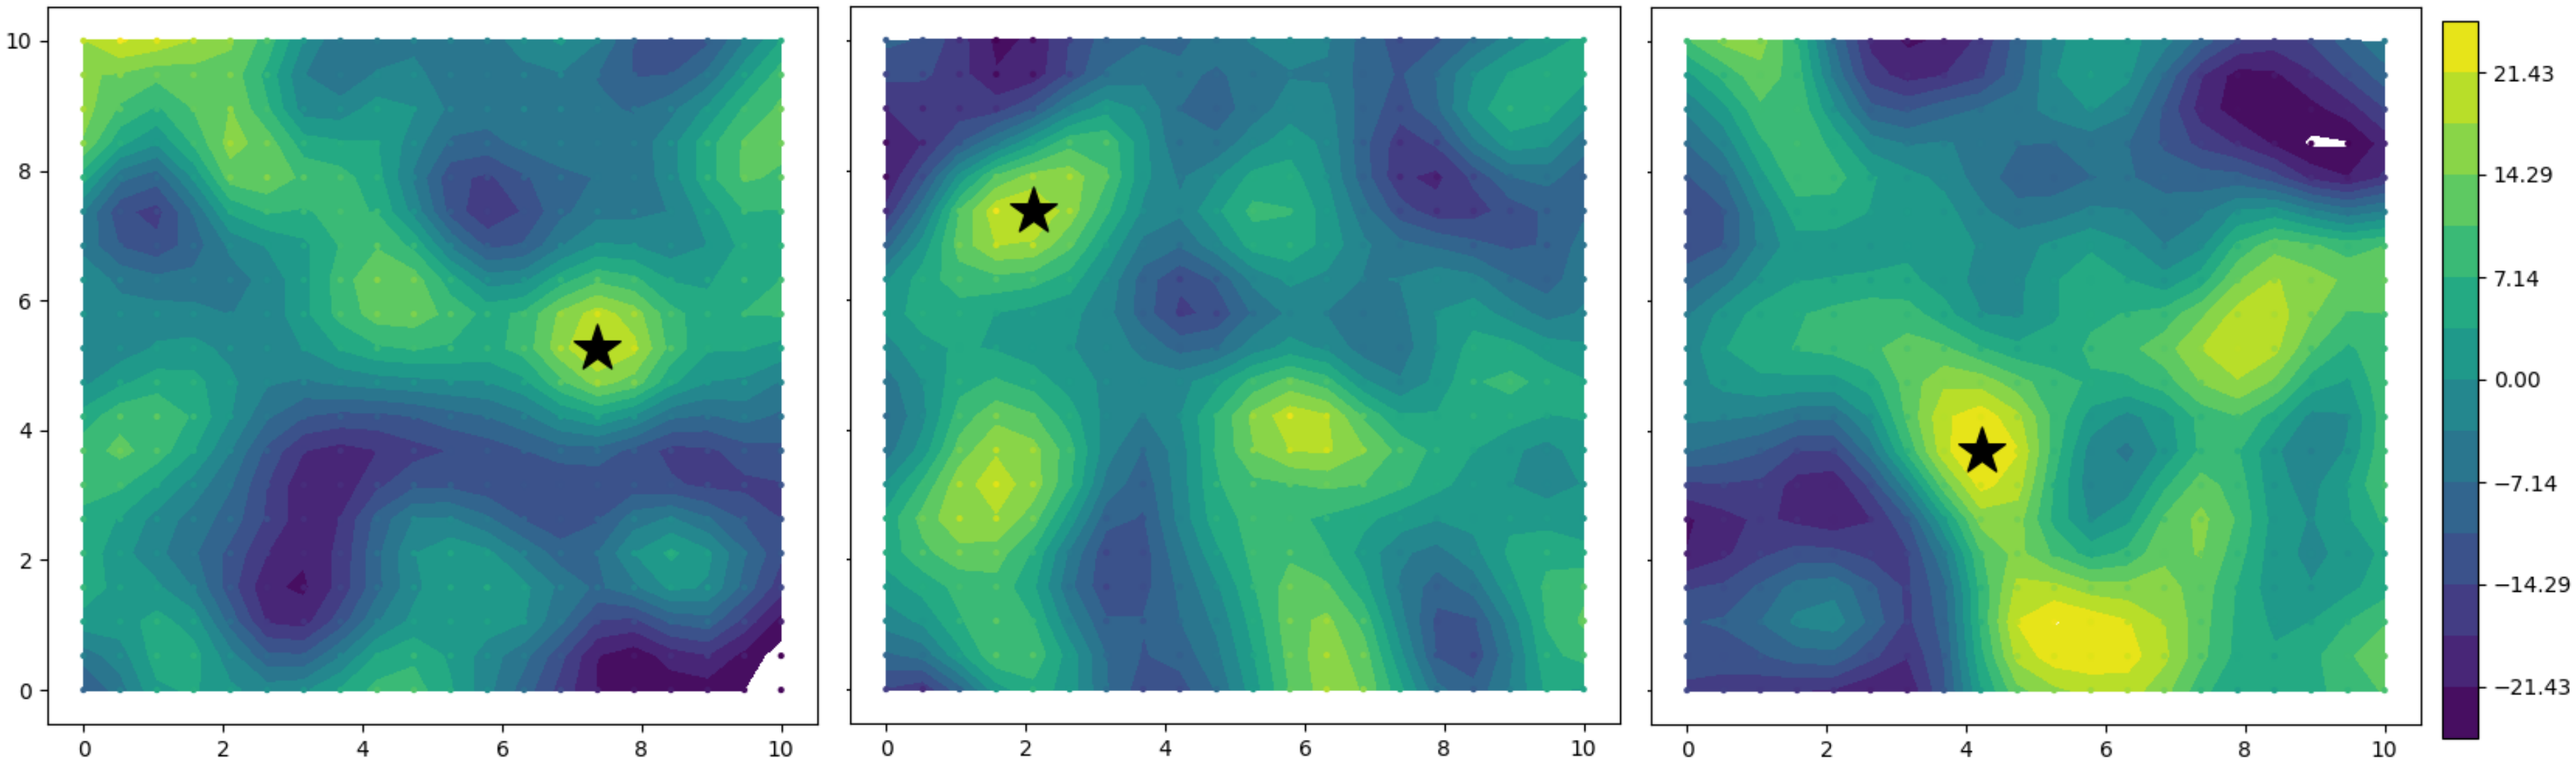
\includegraphics[width=\linewidth]{figures/3sims.png}\hfill
\caption{\textbf{Environments drawn from a Gaussian Process prior:} The complex, multi-modal nature of the simulated environments is evident in these $10$m $\times$ $10$m convex environments. Yellow regions are high-valued; blue regions are low-valued. The global maxima is marked with a star.}
\label{fig:freeworld}
\end{figure}

\subsection{Simulation Parameters}
In all experiments, the environmental domain $\mathbb{X}_w$ is a $10$m $\times$ $10$m square world; several different obstacle scenarios are considered. A random function $f$ representing an environmental phenomena is drawn from a Gaussian Process prior with a squared-exponential covariance function and zero mean function ($l = 1.0$, $\sigma^2 = 100.0$, $\sigma_n^2 = 1.0$ [1\%]). The planning algorithms were provided with these generative hyperparameters; in situations where these are unknown, Bayesian hyperparameter learning can be included in the PLUMES algorithm, as in \cite{wang2017max}. The path-length budget cannot exceed 200m. The fully reachable action set consists of a $20 \times 20$ uniform grid in the world; the limited-horizon action sets are 15 Dubins curves spaced evenly in a circle of radius $1.5$m from $\pm 2.75$ radians (see Figure \ref{fig:obstacles}. The robot moves at a constant velocity and the sampling rate is set such that a sample is collected every $0.5$m. For the nonmyopic planners, a horizon rollout of $5$ actions is used with a computation budget of $150$ rollouts. 

\subsection{Convex Worlds}
\label{sec:free_world}
In the basic simulation scenario, a bounded world with no obstacles is generated. We created 20 random environments for PLUMES and the baseline algorithms to explore. Three example simulated environments are shown in Figure \ref{fig:freeworld}. A table of summary results for the algorithms is presented in Table \ref{tab:free_results}. 

\begin{center}
    
\begin{table}[]
\caption{\textbf{Performance of the algorithms in the convex, obstacle-free world}: Metrics are shown as: mean (std). "Convergence \%" and "Pro. of Samples" denote the percentage of 20 simulations that  converged to within an $\epsilon$-ball of the true global maxima and the proportion of samples collected within that $\epsilon$-ball respectively. Other metrics are as described in Section \ref{sec:metrics}.}
\label{tab:free_results}
\begin{tabular}{l | c | c | c | c | c }
Metric & PLUMES & Myopic PLUMES & Morere et al. \cite{Marchant2014a} & Sun et al. \cite{Sun2017} & Wang et al. \cite{wang2017max}\\ [2pt] 
\hline 
\hline
Convergence \% & \textbf{95.0\%}  & 65.0\% & 55.0\% & 55.0\% & \textbf{95.0\%}\\
Prop. of Samples  & \textbf{0.34} (0.10) & 0.29 (0.21) & 0.26 (0.16) & 0.26 (0.22) & 0.17 (0.03)\\
Net Reward & \textbf{94.8} (15.3) & 82.3 (18.8) & 75.1 (13.2) & 78.0 (19.2) & 88.9 (7.4)\\
$\x^*$ Error & \textbf{0.55} (1.2) & \textbf{0.55} (1.2) & \textbf{0.55} (1.2) & 0.60 (1.2) & 0.57 (1.2) \\
$z^*$ Error & 0.76 (0.5) & \textbf{0.72} (0.5) & 0.75 (0.5) & 0.62 (0.5) & 0.73 (0.4) \\
MSE & 1.46 (0.7) & 1.60 (2.0) & \textbf{1.16} (0.7) & 1.78 (1.9) & 1.39 (1.0) \\
\hline
\end{tabular}
\end{table}
\end{center}
%\begin{figure}[b]
%\centering
%    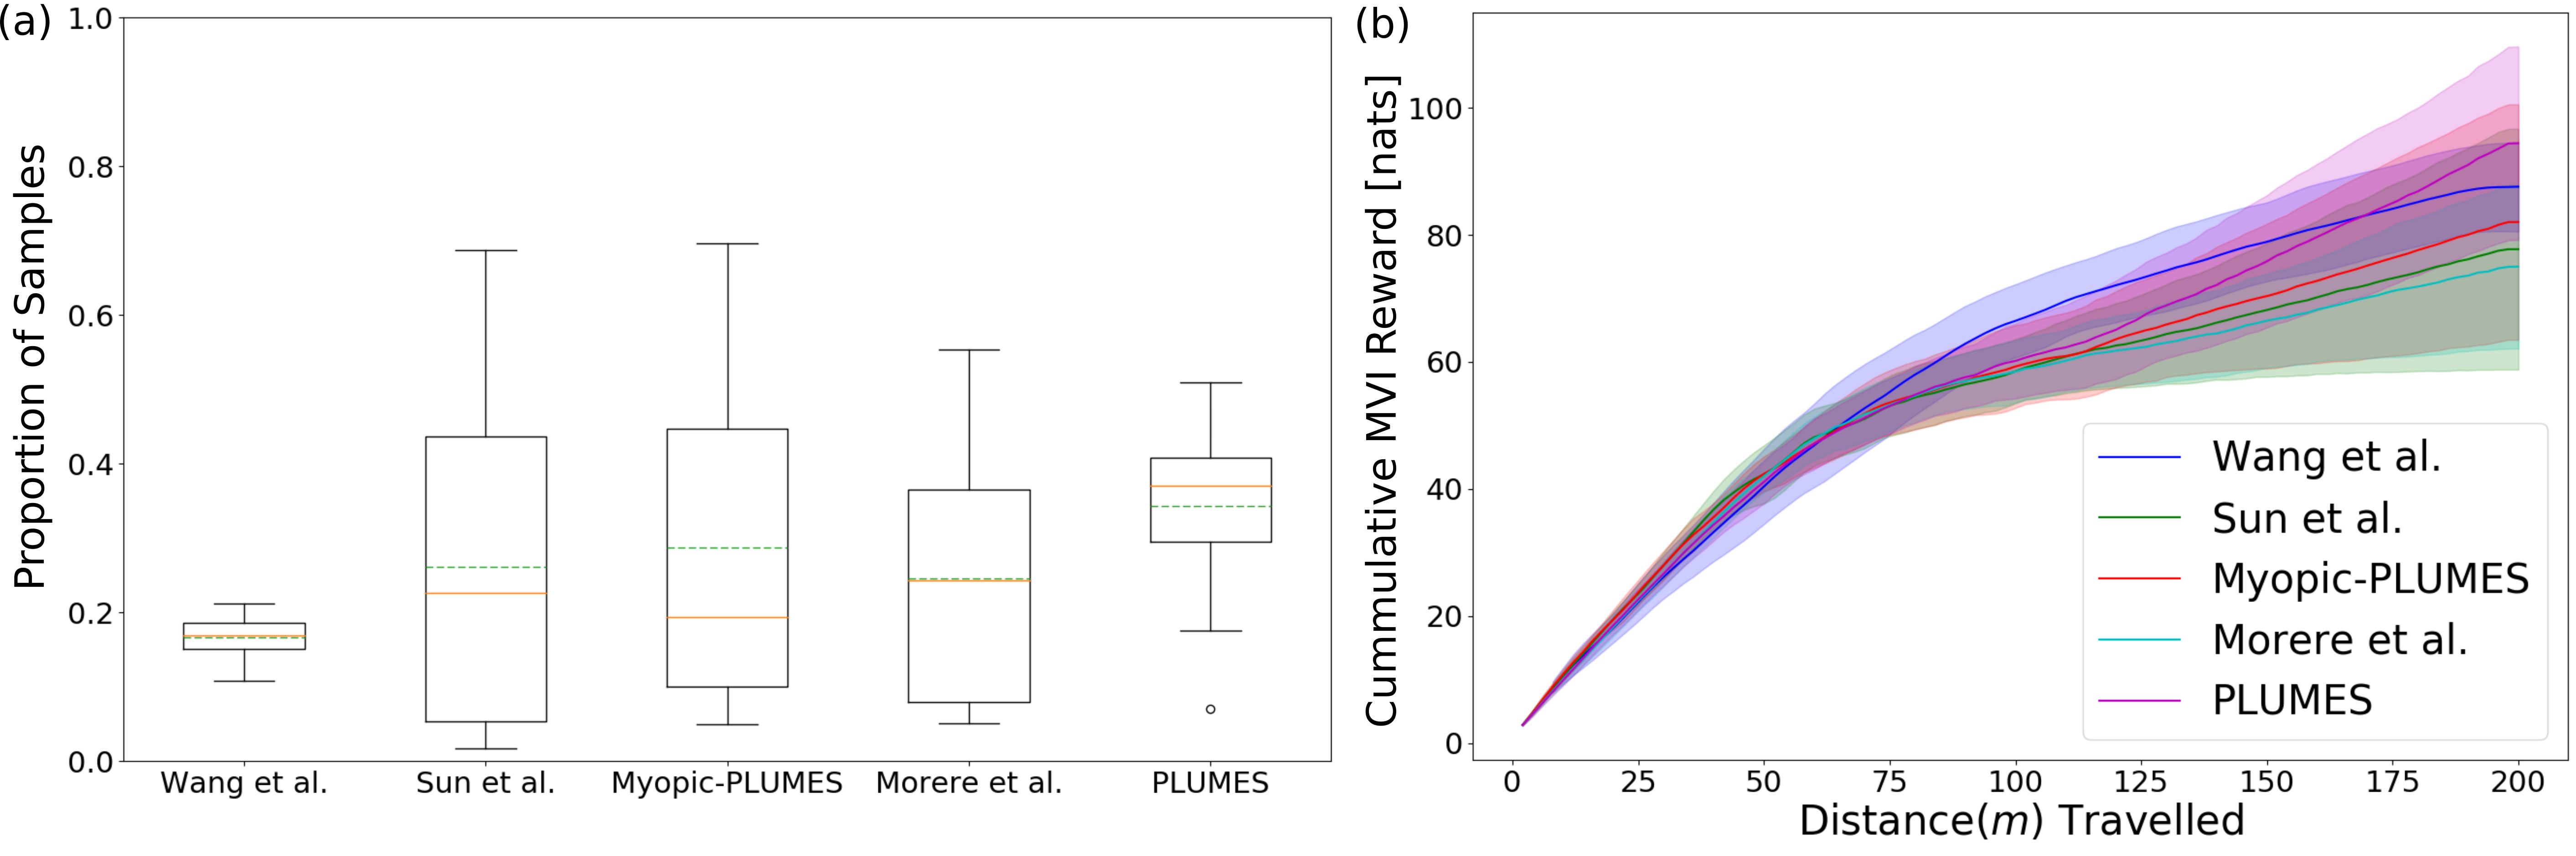
\includegraphics[width=\linewidth]{figures/free_metrics.png}
%    \caption{\textbf{Convergence and reward accumulation for the obstacle-free world:} (a) Proportion of samples in a 200m long trajectory within a 1.5-radius region of the true global maxima. We use this metric as a proxy for indicating location convergence properties. Note that the solid red line is the median, and the dashed green line is the mean of the distribution. (b) The accumulation of MVI reward (Eq. \ref{eq:mves}) over unit distance for each of the algorithms.}    
%\label{fig:free_world}
%\end{figure}


%The convergence behavior of each algorithm is represented in Figure \ref{fig:free_world} (a), along with accumulated reward throughout the duration of the mission in Figure \ref{fig:free_world}(b). 
PLUMES is able to converge to the true global maxima quickly and consistently, collecting the largest proportion of mission samples in an $\epsilon$-ball around the true global maxima, with the second lowest mission-to-mission variation across the 20 simulation experiments.The high convergence success rate for both PLUMES and Wang et al. \cite{wang2017max} signifies that both algorithms were able to consistently localize the true global maxima, but PLUMES collects a much higher proportion of samples around the global maxima, signifying faster convergence for distance-controlled missions. This robust high performance is particularly desirable in real robot systems, for which missions that fail to converge and collect very few samples in the region of interest are a waste of valuable robot time and resources. 




%As all planners are endowed with GP parameters which are good matches to the true underlying phenomenon, the localization estimate is similar. Among planners which use MVI, PLUMES performs well and generally consistently.

%In this world, the empirical results seem to motivate the use of PLUMES for consistency and generally better performance than the other methods. 

\subsection{Environments with Obstacles}
To demonstrate algorithm performance in more complex environments and to highlight some advantages to nonmyopic planning, we generate 20 simulations of each of three types of environments containing obstacles (see Figure \ref{fig:obstacles}):
\begin{itemize}
\item \textbf{Partitioned Environments:} The true maxima of the environment lies on one side of a partition, placed vertically so as to divide the world into proportions of approximately 1/3 and 2/3. A small opening in the partition in the top half of the wall is sized to allow the robot to safely traverse.
\item \textbf{Cloistered Environments:} A room is populated inside of the bounded region, such that the room has three sides, and is only accessible from one side. The environments were generated such that the maxima were placed inside and outside the room).
\item \textbf{Cluttered Environments:} As an extreme robustness test, we generate $10$ environments with many small obstacles placed randomly in the bounded region, such that the robot is able to navigate to anywhere in the environment, but may need a complex trajectory to do so. 
\end{itemize}

In such environments, myopic planning may perform arbitrarily poorly for some configurations of obstacles and global maxima location; whereas nonmyopic planning should be robust to these more adversarial conditions. 
%Empirically, we see support for this in the results.
We repeat the evaluation done in Section \ref{sec:free_world} for environments with these obstacles, and compare PLUMES and the baselines using the metrics discussed. Results for the partitioned and cloistered environments are provided in Table \ref{tab:obstacle_results}. 

\begin{figure}[]
    \centering
    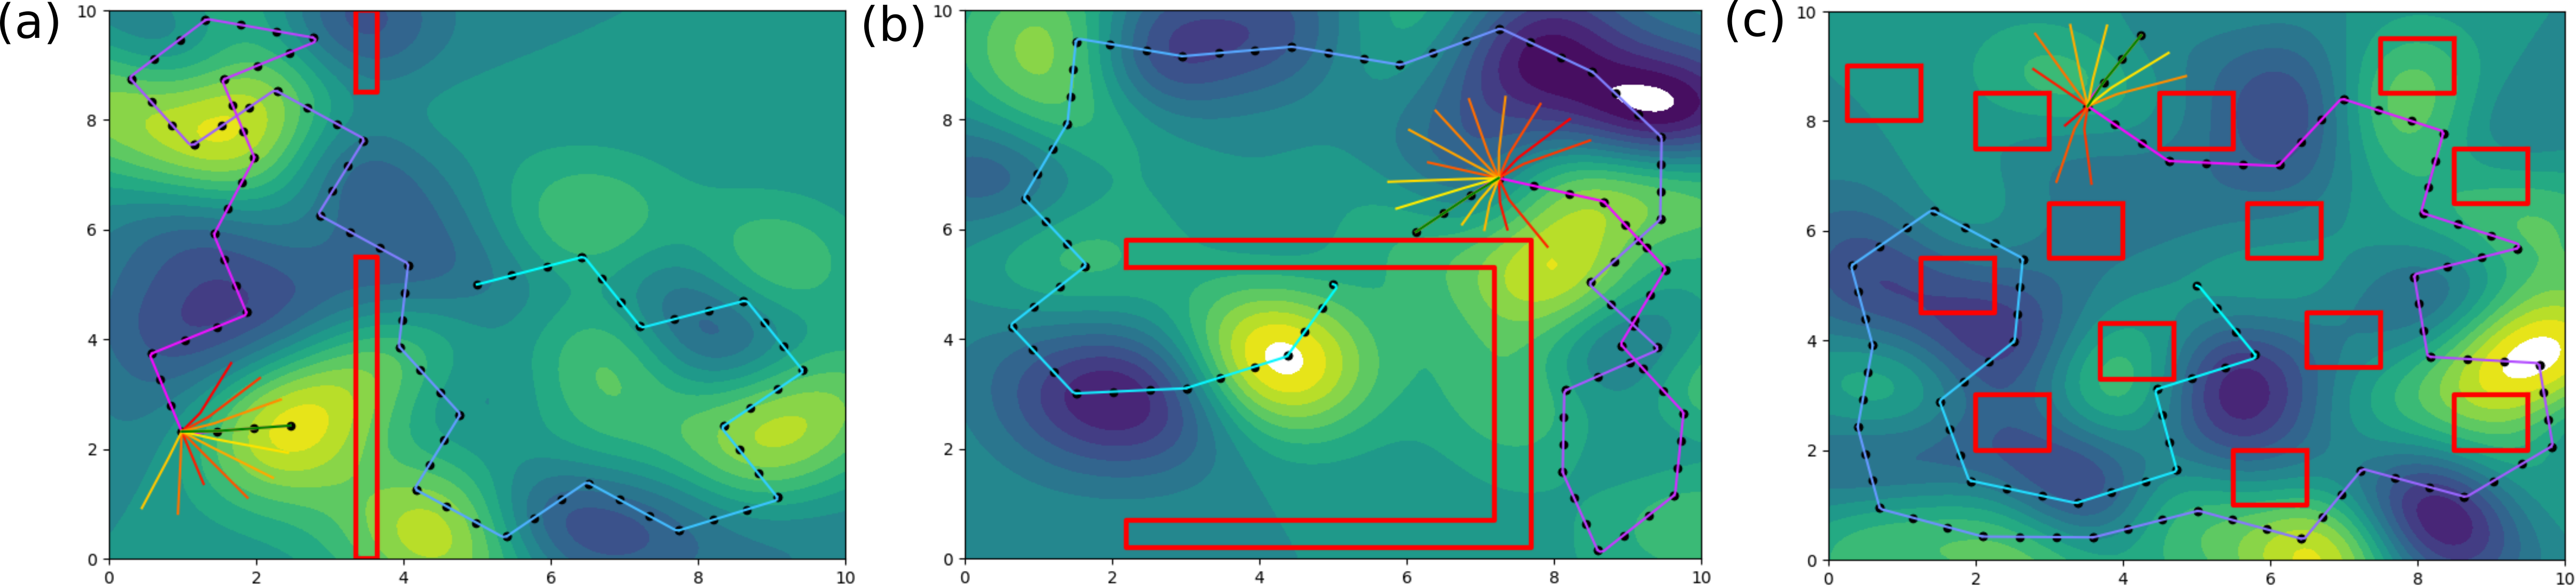
\includegraphics[width=\columnwidth]{figures/3obstacles.png}
        \caption{\textbf{Simulated environments containing obstacles:} Simulated worlds are shown with partial trajectories constructed by a limited-horizon robotic planner. Collected samples appear as black dots. Parts of the trajectory colored blue are earlier in the mission; parts colored pink are more recent. The current set of actions available to the robot is illustrated, as well as the selected action. The robot's current belief on the function $f$ is shown in the background.  (a) Illustrative figure of the partition world, in which the partition is represented by the red boxes. (b) The cloistered environment. (c) The cluttered environment.}
    \label{fig:obstacles}
\end{figure}

\begin{table}[b]
\caption{\textbf{Performance of the algorithms in the partitioned and cloister environments}: Metrics are shown as: mean (std). "Convergence \%" and "Pro. of Samples" denote the percentage of 20 simulations that  converged to within an $\epsilon$-ball of the true global maxima and the proportion of samples collected within that $\epsilon$-ball respectively. Other metrics are as described in Section \ref{sec:metrics}.}
\label{tab:obstacle_results}
\begin{tabular}{l | c | c | c | c | c }
Metric & PLUMES & Myopic PLUMES & Morere et al. \cite{Marchant2014a} & Sun et al. \cite{Sun2017} & Wang et al. \cite{wang2017max}\\ [2pt] 
\hline 
\hline
Convergence \% & \textbf{95.0\% } & 70.0\% & 50.0\% & 65.0\% & 85.0\% \\ Prop. of Samples  & \textbf{0.36} (0.12)  & 0.29 (0.23) & 0.17 (0.22) & 0.26 (0.22) & 0.25 (0.10) \\
Net Reward & 93.1 (18.7) & 75.2 (19.8) & 68.1 (17.9) & 68.4 (19.0) & \textbf{101.5} (20.2)\\
$\x^*$ Error & 0.59 (1.2) & 0.59 (1.2) & 0.82 (1.5) & 1.38 (2.2) & \textbf{0.56} (1.3) \\
$z^*$  Error & 0.73 (0.5) & 0.69 (0.5) & 0.59 (0.5) & 1.22 (1.3) & \textbf{0.68} (0.5) \\
MSE & 2.48 (2.1) & 6.44 (9.8) & 7.01 (11.3) & 12.4 (17.8) & \textbf{1.97} (1.6) \\
\hline
\end{tabular}
\end{table}

PLUMES accumulates nearly the same amount of MVI reward as Wang et al. \cite{wang2017max}. Additionally, PLUMES is able to successfully converge to the global maxima in more environments compared to baseline algorithms and gathers more than a third of the samples taken within an $\epsilon$-ball of the global maxima. The proportion of samples taken near the global maxima for each algorithm in the partition and cloistered environments is visualized in Figure \ref{fig:obstacle_results}.
%from this figure, PLUMES speed of convergence to the global maxima is eviden(the middle 50\% of the data largely fall in the upper 50\% or higher of the baselines and PLUMES has a much smaller inter-quartile range (IQR)). 
The maxima location and value estimation is comparable among all the algorithms. The Myopic PLUMES and Sun et al. algorithms both suffer from high MSE, which indicates an occasional degenerate case in which these algorithms arbitrarily converge to an estimated local maxima before the whole of the reachable world is explored. 

\begin{figure}[t]
\centering
    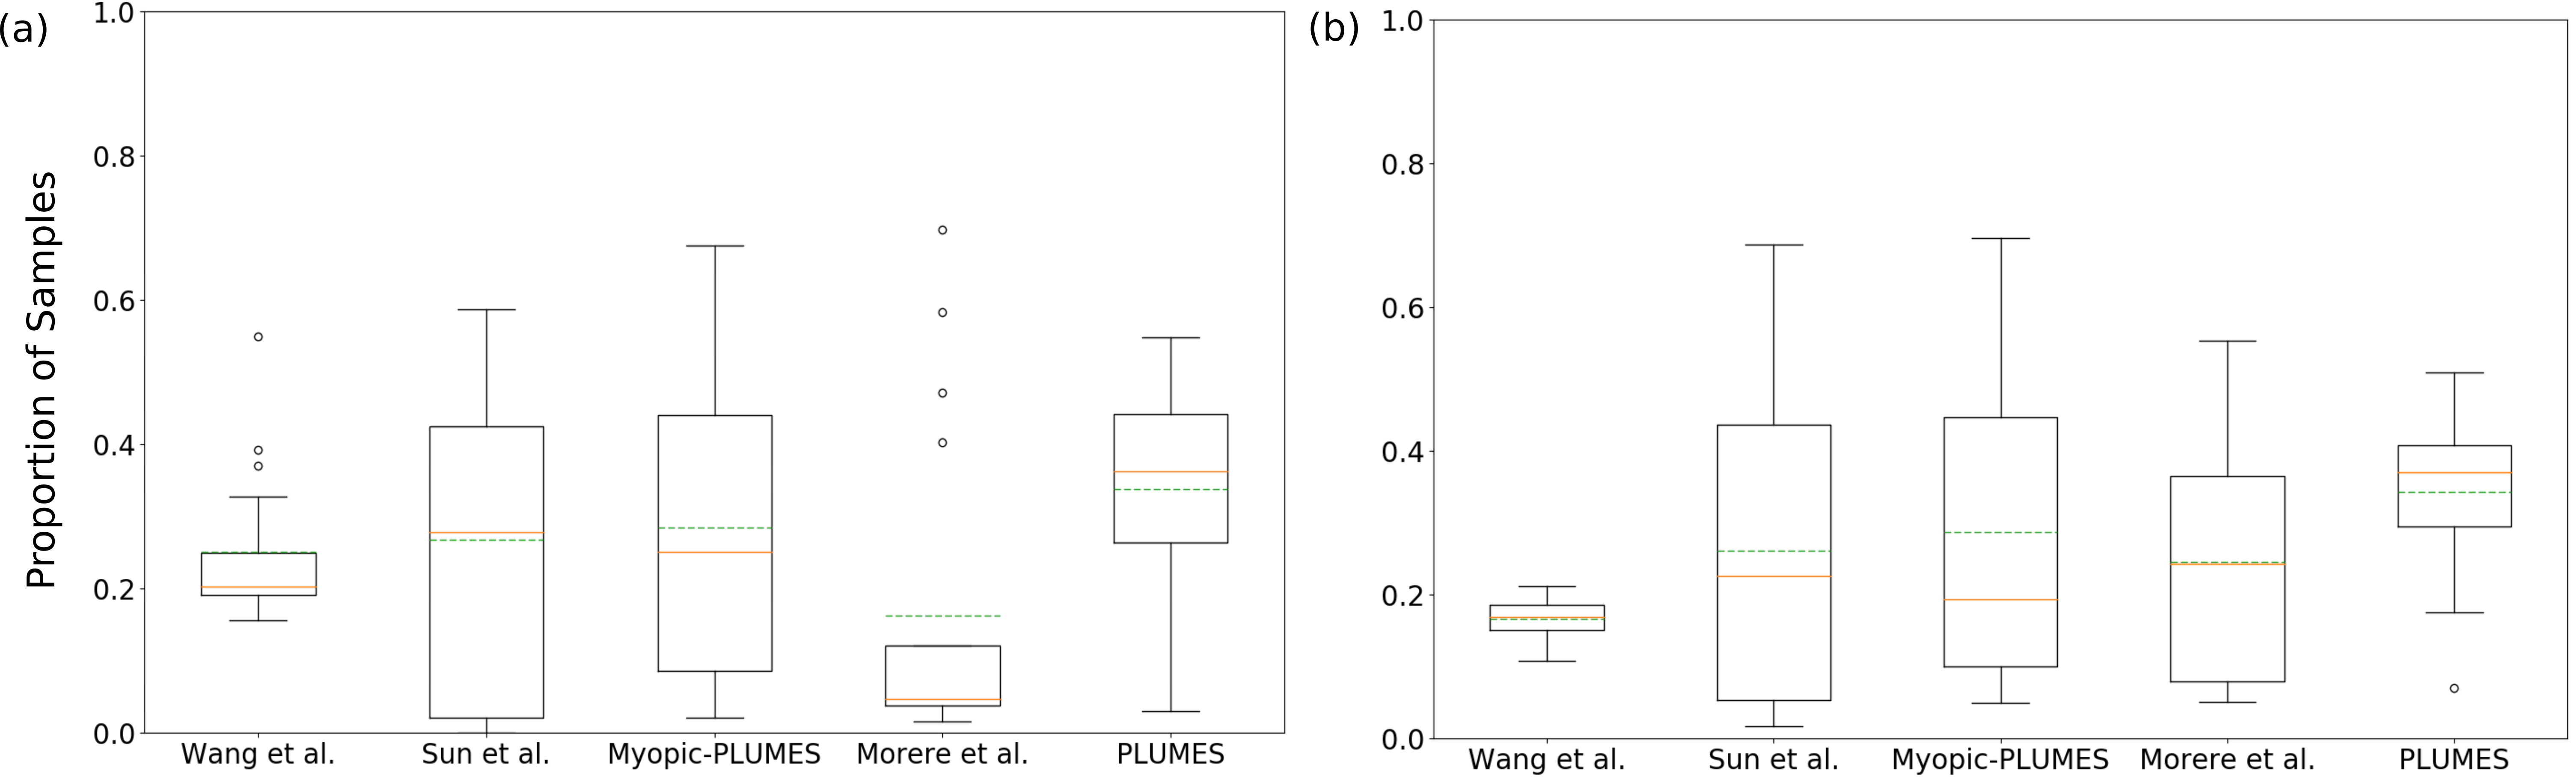
\includegraphics[width=\linewidth]{figures/obstacle_props.png}
    \caption{\textbf{Convergence for the obstacle environments:} The proportion of samples in a 200m long trajectory within a 1.5-radius region of the true global maxima. We use this metric as a proxy for indicating location convergence properties. Note that the solid red line is the median, and the dashed green line is the mean of the distribution. (a) The partitioned environment. (b) The cloistered environment.}    
    \label{fig:obstacle_results}
\end{figure}


For the challenging, adversarial cluttered environment, we evaluate the number of successful convergences to the true global maxima for each algorithm, presented in Table \ref{tab:cluttered}. PLUMES is able to converge to the global maxima with an impressive 100\% success rate in $10$ random environments. This cluttered environment demonstrates the potential for arbitrary failure cases for myopic planners. The modified myopic Wang et al. algorithm is able to still successfully converge in 8 of the 10 trials due to it's rich action set. However, this size of the action set makes nonmyopic extensions to the Wang et al. algorithm unfeasible, which in turn leads to arbitrary failures in complicated environments. The trajectories constructed by each planning algorithm in an example cluttered environment is shown in Figure \ref{fig:cluttered_ex}.

\begin{table}[h]
\caption{\textbf{Mission success in cluttered environment}: The percentage of 10 simulations that converged to within an $\epsilon$-ball of the true global maxima.}
\label{tab:cluttered}
\begin{tabular}{l | c | c | c | c | c }
Metric & PLUMES & Myopic PLUMES & Morere et al. \cite{Marchant2014a} & Sun et al. \cite{Sun2017} & Wang et al. \cite{wang2017max}\\ [2pt] 
\hline 
\hline
Convergence \% & \textbf{100.0\% } & 40.0\% & 30.0\% & 30.0\% & 80.0\% \\
\hline
\end{tabular}
\end{table}


\begin{figure}[t]
\centering
    \includegraphics[width=\linewidth]{figures/cluttered_ex.png}
    \caption{\textbf{Trajectories for the cluttered environment:} Final trajectories for the five planning environments. Collected samples appear as black dots. Parts of the trajectory colored blue are earlier in the mission; parts colored pink are more recent, allowing final convergence to be more easily visualized. The robot's current belief on the function $f$ is shown in the background.  (a) The unknown ground-truth environmental model, with the global maxima denoted with a star and obstacles shown. (b)-(f): The final trajectory and belief model for PLUMES and the baseline algorithms. Only PLUMES is able to successfully converge to and densely sample the global maxima.}    
    \label{fig:cluttered_ex}
\end{figure}


%\begin{table}[H]
%\caption{Performance of the algorithms in the partition world}
%\label{tab:partition_results}
%\begin{center}
%\noindent
%\begin{tabular}{l | c | c | c | c | c }
%Metric & PLUMES & Myopic PLUMES & Morere et al. [?] & Sun et al. [?] & Wang et al. [?]\\[2pt]
%\hline
%\hline\rule{0pt}{12pt} 
%MSE & (1.36, 1.1) & (7.95, 10.6) & (1.34, 1.0) & (9.55, 11.5) & (2.17, 3.0) \\
%Location Error & (0.55, 1.2) & (0.55, 1.2) & (0.75, 1.4) & (0.69, 1.3) & (0.53, 1.2) \\
%Value Error & (0.73, 0.5) & (0.67, 0.5) & (0.73, 0.4) & (1.21, 2.1) & (0.70, 0.5) \\
%Net Reward & (92.46, 17.9) & (80.24, 19.4) & (71.80, 11.7) & (79.15, 24.4) & (99.29, 25.6)\\
%\hline
%\end{tabular}
%\end{center}
%\end{table}


%The sampling density is represented in Figure \ref{fig:partition_density}. Generally, the distribution of the performance with respect to sample proportion indicates the PLUMES performs somewhat consistently, with the middle 50\% of the data largely falling in the upper 50\% or higher to the baselines. 
%As a final analysis, we observe the rate of reward accumulation over unit distance in Figure \ref{fig:partition_reward}. \textbf{PENDING RE-ANALYSIS OF FIGURE. Once complete, we expect to see that Wang et al. will grow at a rate more quickly than PLUMES, but they will begin to look similar as distance increases towards the budget limit}. 


%Generally, the performance of all of the algorithms with regards to localization and convergence in this world is impacted as compared to the convex, obstacle-free environment. PLUMES is somewhat robust to this more adversarial environment, maintaining good exploration and convergence properties, attractive for this problem.


%Now, we explicitly compare PLUMES and the baselines using the metrics discussed. Table \ref{tab:cloister_results} is provided.

%\begin{table}[H]
%\caption{Performance of the algorithms in the partition world}
%\label{tab:cloister_results}
%\begin{center}
%\noindent
%\begin{tabular}{l | c | c | c | c | c }
%Metric & PLUMES & Myopic PLUMES & Morere et al. [?] & Sun et al. [?] & Wang et al. [?]\\[2pt]
%\hline
%\hline\rule{0pt}{12pt} 
%MSE & (2.48, 2.1) & (6.44, 9.8) & (7.01, 11.3) & (12.40, 17.8) & (1.97, 1.6) \\
%Location Error & (0.59, 1.2) & (0.59, 1.2) & (0.82, 1.5) & (1.38, 2.2) & (0.56, 1.3) \\
%Value Error & (0.73, 0.5) & (0.69, 0.5) & (0.59, 0.5) & (1.22, 1.3) & (0.68, 0.5) \\
%Net Reward & (93.15, 18.7) & (75.25, 19.8) & (68.17, 17.9) & (68.41, 19.0) & (101.54, 20.2)\\
%\hline
%\end{tabular}
%\end{center}
%\end{table}

%These results generally corroborate what was observed in the partition world. It is interesting to note that the performance of the Wang et al. approach is still quite good, despite the adversarial conditions and myopic planning horizon. The size and richness of the pathsets provided may be partially responsible for this behavior.

%The sampling density is represented in Figure \ref{fig:cloister_density}. Generally, the distribution of the performance with respect to sample proportion indicates the PLUMES performs somewhat consistently, with the middle 50\% of the data largely falling in the upper 50\% or higher to the baselines. 


%We observe further observe the rate of reward accumulation over unit distance in Figure \ref{fig:cloister_reward}. \textbf{PENDING RE-ANALYSIS OF FIGURE. Once complete, we expect to see that Wang et al. will grow at a rate more quickly than PLUMES, but they will begin to look similar as distance increases towards the budget limit}. 




%%%%%%%%%%%%%%%%%%%%%%%%%%
%%%% RELATED WORKS
%%%%%%%%%%%%%%%%%%%%%%%%%%
\section{Related Work}
\label{sec:related_works}
%\textbf{In Progress: Previous related works from CORL draft needs to be heavily edited, but much of the content is the same. Also unclear how in depth we should go into literature for each discrete part (UCT-MCTS, MVI, UCB, Myopic Paths, etc). Advice appreciated.}

Information-gathering in unknown environments is of widespread interest in a variety of domains, including sensor selection \cite{Krause2008, KrauseDanielGolovin, Srivastava2011}, active simultaneous localization and mapping (active-SLAM) \cite{Sim2004, Charrow2015, Charrow2015a, Cadena2016}, active machine learning \cite{Zhu2010}, optimal experimental design \cite{Lorenz2015}, and Bayesian optimization \cite{Inza2000, Boender1987}. For robotic platforms, the combination of information-gathering with path planning leads to unique optimization challenges when considering limitations of the physical platforms, such as dynamics, sensing-frequency, path-cost, etc. 
%Presented in this paper is a nonmyopic MCTS strategy that utilizes a novel MVI reward acquisition function in order to identify and converge upon a true global optima in unknown environments. 

The concept of using nonmyopic planning horizons with information-theoretic reward functions is a well-established principle. When the information-theoretic reward functions do not depend on realized observations, such as in a Gaussian process with pure information-gain reward, a number of solutions have exploited the submodularity of information gain for near-optimal myopic sensor placement \cite{Krause2008}.  When the reward function does depend on realized observations, solutions must trade-off exploration and exploitation. One of the baselines in this work, Morere et al.'s sequential Bayesian optimization MCTS with UCB-reward function, illustrates the empirical advantages of the method; and a number of works have expounded on putting bounds on the performance of UCT-MCTS with UCB reward functions \cite{Patten2018, Katt2017, ling2016gaussian} in discrete POMDP formulations \cite{Silver2010}. However, as demonstrated in this paper, UCB-based planners can suffer from poor finite-time performance for the task of global maxima localization, even in simple simulation experiments. %To date, there has been no work to analyze the efficacy of MVI as a suitable reward function to establish equivalent bounds on performance given the same assumptions in planning. 

Solving bounds for a discrete POMDP is non-trivial, however, by using a GP as the means for calculating online updates to a POMDP, observations are no longer discrete quantities.  To work around continuous domains in POMDP planning with GPs, one strategy is to abstract, bin, or otherwise discretize continuous observations and state spaces. \cite{ling2016gaussian} in particular abstracts observations made in a GP to have a discrete, deterministic value and assumes  Lipschitz continuous reward function, thus allowing for a bound on the optimality of the planning solution. Discretizing in this way is problem dependent, and selecting good parameters for discretization is not necessarily intuitive for many problem contexts. By drawing on fundamental principles of prediction error in GPs \cite{Wagberg2017} and classical analysis on MCTS \cite{Kocsis2006} this work illustrates that continuous observation space can be used in nonmyopic POMDP solutions, and the performance bounded (hopefully:)). Such a strategy has been claimed in works like \cite{Arora2017}, however, a rigorous analysis of the claim with the MVI reward-acquisition function, has yet to have been demonstrated. 

Indeed, the Upper Confidence Bound (UCB) acquisition function is perhaps the most prevalent metric and is used in multiple information planning domains \cite{Carpentier2011, Contal2013, Srinivas2012a}. It was only more recently, the Bayesian optimization community began to refocus efforts on the entropy search acquisition functions for black-box function optimization \cite{hennig2012entropy, hernandez2014predictive, wang2017max} that explictly try to reduce model entropy around the global maxima. Until the work of \cite{wang2017max} which introduced significant computational performance gains over other entropy-search methods, these acquisition functions would have been very costly or difficult to compute on a robotic platform. The no-regret properties of Wang et al., which has been shown to have proven comparable performance to UCB for certain settings of UCB's free parameter $\beta$ \cite{wang2016optimization}, make it an attractive reward function robotic-planning problems. 




%%%%%%%%%%%%%%%%%%%%%%%%%%
%%%% CONCLUSIONS, FUTURE WORK
%%%% Outline: Wrap up, re-iterate contributions, note limitations and move into open areas (continuous space, non-convex space, non-myopic strategies, etc)
%%%%%%%%%%%%%%%%%%%%%%%%%%
\section{Discussion and Future Work}
\label{sec:discussion}
%In a convex world with unique local maxima, the planners with MVI acquisition function empirically tend to outperform those which are UCB-based with regards to convergence metrics. Intuitively, through the process of spectral sampling, the MVI acquisition function has implicitly encoded information about the distribution of the environment and the true value of the maximizer $z*$, and gains reward with respect to this information. UCB reward, however, is only accumulated with respect to local observation.
Developing online planning methods for optima seeking and convergence are critical for practical use of robotic platforms in a variety of contexts, including general environmental monitoring (scientific inquiry, reconnaissance) and disaster-response (oil spill, gas leak, radiation). By uniting and advancing several state of the art methods, PLUMES is able to demonstrate the effective and robust finite-time convergence properties that are very attractive for practical domains. 

We want to highlight several key observations from our theoretical and empirical results. Firstly, our experimental results demonstrate that the maximum-value information reward, MVI, is a robust alternative to UCB for localization and monitoring of the global maxima of an \textit{a priori} unknown environment using mobile robotic platforms. In all simulation results, the MVI-based planning algorithms outperformed the equivalent UCB-algorithm in both maximum-value information gain and speed/robustness of convergence to the global maxima e.g. PLUMES outperformed the UCB-based nonmyopic planner in Morere et al.; myopic PLUMES outperformed the UCB-based myopic planner in Sun et al.

Recent work in robot maxima finding in continuous environments has focused on robots with discrete, local action sets, parameterized by Dubins curves, or splines [CITE] and UCB-based acquisition functions. However, our results suggests that using UCB in combination with local actions sets can lead to poor finite-time performance for both myopic and nonmyopic planning horizons. Myopic methods that employ UCB, build global Gaussian process belief maps of the unknown function $f$, but only use local evaluations to estimate the reward of potential actions i.e. our experiments show that all algorithms were able to accurately estimate $\x^*$ and $z^*$ early in the mission; the UCB-algorithms had no way to use these estimates to prevent getting stuck gathering sub-optimal reward in a local maxima.  Alternatively, MVI uses the global model belief to explicitly generate samples of the global maxima $z^*$ and uses this knowledge to adaptively trade-off exploration and exploitation. %Empirically, when the planning horizon was made to be nonmyopic, MVI continued to outperform UCB for finite-length missions, which is posited to be the result of the combination of global sampling with global planning for MVI, as opposed to more greedy mean accumulation in the UCB approach. 
For Gaussian process belief models, MVI presents a principled, parameter-less way to \textbf{incorporate global information to guide local search} and manage the exploration-exploitation trade-off. 
%The performance analysis presented argues that the use of MVI is a good approximation for true optima identification, and within the PLUMES algorithm, is able to maintain asymptotic optimality guarantees under nonmyopic planning. Empirically, MVI-based planning schemes outperform the twin scheme with UCB reward acquisition function. We leave it as future work to more tightly bound and predict the performance of PLUMES, and myopic-planners that utilize MVI. 

Nonmyopic planning with constrained action sequences is a computationally suitable alternative to highly-discretized myopic planning with added benefit to extending optima seeking to nonconvex environments. Although the myopic approach of Wang et al. \cite{wang2017max} performed consistently well, the size of the action set $\mathcal{A}$ required is $O(N^d)$ for environments of dimension $d$, making nonmyopic planning computationally unfeasible.  Using a significantly reduced action set ($\left\vert \mathcal{A} \right\vert = 15$) with a UCT-MCTS nonmyopic planner, we are able to construct trajectories that converge more quickly to the global maxima, and additionally demonstrate robust convergence and information gathering in complicated environments with adversarial obstacles. 

%Several of the naive, degenerative cases discussed may be suitable platforms for future development for myopic trajectory optimization. Particularly attractive is a modified cost-benefit ratio reward function; which although we demonstrated can perform arbitrarily poorly, the empirical behavior in successful cases scored highly on the metrics of interest we presented here.

Ultimately, PLUMES motivates the use of restricted action sets in a nonmyopic planning framework that uses UCT-MCTS with a novel MVI reward-acquisition function to perform maximum-value information gathering in \textit{a priori} unknown environments with adversarial conditions (multiple local maxima, presence of obstacles, limited travel budget). We perform novel analysis to show asymptotic convergence guarantees for the performance of PLUMES, and present empirical evidence that MVI-based planners are be a robust alternative to state of the art UCB-based methods.
%
% ---- Bibliography ----
%
\bibliographystyle{IEEEtran}
\bibliography{ipp}
\end{document}
